\documentclass{standalone}
\usepackage{tikz}
\usetikzlibrary{intersections, calc}
\usepackage{hsbcommon}
    \begin{document}
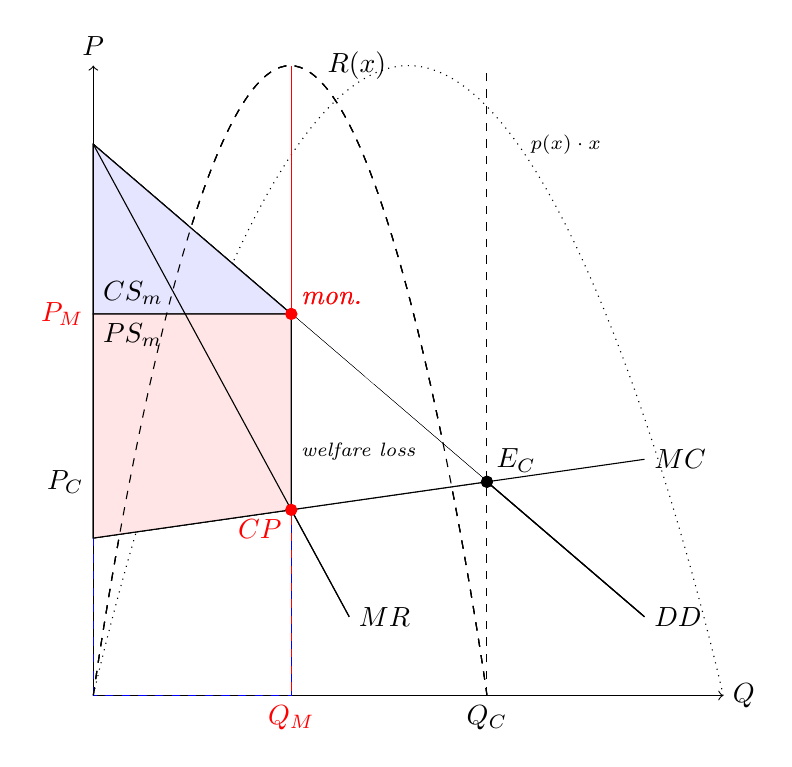
\begin{tikzpicture}[remember picture]
        \draw[->] (0,0) node[below] {\phantom{$X_i$}} -- (8,0) node[right] (Q) {$Q$};
        \draw[->] (0,0) node[left] {\phantom{$Y_mi$}} -- (0,8) node[above] (P) {$P$};

        \coordinate (A) at (0,7);
        % \coordinate (B) at (2,6);
        % \coordinate (C) at (3,4);
        % \coordinate (D) at (4,3);
        % \coordinate (E) at (6,2);
        \coordinate (F) at (7,1);
 
        \draw [name path=demand] plot [smooth] coordinates {(A) (F)};
        \node[right] at (F) {$DD$};

        % Demand curve

        \coordinate (G) at (0,2);
        % \coordinate (H) at (2,3);
        % \coordinate (I) at (3,3);
        % \coordinate (J) at (5,3);
        % \coordinate (K) at (6,3);
        \coordinate (L) at (7,3);
        
        \draw [name path=supply] plot [smooth] coordinates {(G) (L)};
        \node[right] at (L) {$MC$};

        \ifstep{1}{
        
        %% COMPETITION CASE
            
            \path [name intersections={of=demand and supply,by=X}];
    
            \filldraw (X) circle (2pt) node[above right] {$E_C$};
    
            % \draw[dashed, red] (0,0) rectangle (X);
            
            \draw [dashed] (X |-, 0) node[below] {$Q_C$}-- (X |-, 8);
            \draw[dotted] (X) -- (0, |- X) node[left] {$P_C$};

            \draw [fill=blue!10] (X)  -- (0, |- X) --   (A) node [below=20pt, right] {$CS$} ;
            \draw [fill=red!10] (X) -- (0, |- X) -- node [right] {$PS$}  (G);
            
        }

        \ifstep{2}{

            \foreach [count=\i] \myvalue/\mycolor in {0.5/red,0.18/blue}
            {
            \coordinate (M\i) at ($(A)!\myvalue!(F)$);
            \path[name path=m1] (0, |- M\i) -- (M\i) -- (M\i |-,0);
            \path [name intersections={of=m1 and supply,by=myy}];
            \filldraw[\mycolor] (M\i) node[below left] {\scriptsize  $P_\i$} circle (1.5pt);
            % \filldraw (myy) circle (2pt);
            \draw[thick,\mycolor] (M\i) -- ([yshift=\i pt]myy) -- ([xshift=\i pt,yshift=\i pt]G) -- ([xshift=\i pt]0, |- M\i) node[below right ] {$PS_\i$} -- cycle;
            }
        }

        \ifstep{3}{

        %%% hide hilfspunkte and re-draw demand curve
 
        \draw [name path=demand] plot [smooth] coordinates {(A) (F)};
        %%%

        %% MONOPOLY CASE
        
            % \coordinate (M) at (0,8);
            % \coordinate (B) at (2,6);
            % \coordinate (C) at (3,4);
            % \coordinate (D) at (4,3);
            % \coordinate (E) at (6,2);

            %% draw profit parablola
            \coordinate (M) at (0,0) ;
            \coordinate (N) at (2.5,8);
            \coordinate (O) at (5,0);
            \draw[dashed] (M) plot [smooth,tension=1] coordinates {(M) (N) (O)};
            \node[right=10pt] at (N) {$R(x)$};
            
            }

        \ifstep{4}{

            %% hide and correct
            \filldraw[white] (M1) circle (2pt);
            \filldraw[white] (M2) circle (2pt);   
            \draw [name path=demand] plot [smooth] coordinates {(A) (F)};            
            \draw [fill=blue!10] (X)  -- (0, |- X) --   (A) node [below=20pt, right] {$CS$} ;
            \draw [fill=red!10] (X) -- (0, |- X) -- node [right] {$PS$}  (G);
            \draw[dashed] (M) plot [smooth,tension=1] coordinates {(M) (N) (O)};

            \draw[dotted] plot [smooth,tension=1] coordinates {(0,0) (4,8)(8,0)}; \node at (6,7) {\scriptsize $p(x)\cdot x$};
            %%%%
            
            \coordinate (Q) at (3.25,1);
     
            \draw [name path global=mr] plot [smooth] coordinates {(A) (Q)};
            \node[right] at (Q) {$MR$};
        
            \path [name intersections={of=mr and supply,by=Y}];
            \filldraw[red] (Y) circle (2pt) node[below left] {$CP$};
    
        }

        \ifstep{5}{
\begin{scope}[color=red]
   
    
            \draw [name path=mono] (Y |-, 0) node[below] {$Q_M$} -- (Y |-, 8);
            \path [name intersections={of=mono and demand,by=Z}];
            
            \filldraw (Z) circle (2pt) node[above right] {\textit{mon.}};
            \draw (Z) -- (0, |- Z) node[left] {$P_M$};
    
        \end{scope}
}

        \ifstep{6}{

            
            \draw [fill=white] (X) -- (G) -- (A);
            \draw[dashed, blue] (0,0) rectangle (Y);
            
            \draw [fill=blue!10] (Z) -- (0, |- Z) node [above right] {$CS_m$} --   (A)  --  cycle;

            
            \draw [fill=red!10]  (0, |- Z) node[below right] {$PS_m$}   --  (Z) -- node[right,yshift=-0.5cm] {\scriptsize \textit{welfare loss}}  (Y) --  (G) -- cycle;
            \draw [name path=mr] plot [smooth] coordinates {(A) (Q)};
            \filldraw (X) circle (2pt);
            \filldraw[red] (Z) circle (2pt) node[above right] {\textit{mon.}};
            \filldraw[red] (Y) circle (2pt) ;
                        \draw[dashed] (M) plot [smooth,tension=1] coordinates {(M) (N) (O)};0        }

        
        
    \end{tikzpicture}
\end{document}
